84. $y=\left|\cfrac{3+x}{6}
ight|=\begin{cases}\cfrac{x+3}{6},\ x\geqslant-3\\ \cfrac{-x-3}{6},\ x<-3.\end{cases}$
$$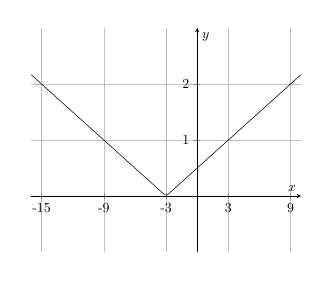
\begin{tikzpicture}[scale=0.5]
\begin{axis}[
    axis lines = middle,
    grid=major,
    legend pos={south west},
    xlabel = {$x$},
    ylabel = {$y$},
    ymin=-1,
    ymax=3,
    xtick={-15,-9,-3,3,9},
    xticklabels={-15,-9,-3,3,9},
    ytick={1,2},
    yticklabels={1,2}            ]
	\addplot[domain=-16:10, samples=100, color=black] {abs((3+x)/6)};
%\addplot[domain=1:6, samples=100, color=black] {x*x-4};
%\addplot[domain=-3.1:2.5, samples=100, color=red] {70*abs(1-2*abs(abs(x)-2))-10*x^2+10*x-70};
	%\addlegendentry{$\text{Рис. 1}$};
\end{axis}
%\draw (3.47,1.89) circle (2pt);
%\draw (3.47,0.63) circle (2pt);
\end{tikzpicture}$$
Исходя из графика, найдём ответ $x\in[-15;9].$\\
